\graphicspath{{Chapters/ObjEventSelection/Figures/}}
\chapter{Object and Event Selection}
\label{chap:ObjEventSelection}

\section{Electron Selection}
\label{sec:objsel-el}

Electron reconstruction and identification was described in~\sec{reco-el}. Both
central electrons with \modetalt{2.47} and forward electrons are used. In
addition to the identification requirements described in~\sec{reco-el}
additional selection requirements are imposed to select electrons likely to have
originated from \Z\ boson decays and to reject backgrounds. The requirements are
slightly different for the 8 \tev\ analysis compared to the 7 \tev\ analysis,
reflecting the different experimental conditions (such as higher pile-up in
2012) as well as optimisations made in 2012. The electron selection requirements
are summarised in~\tab{objsel-el} are described in more detail below. 

\begin{table}[]
  \centering
%   \vspace*{-1cm}
%\small
  \begin{tabular}{ l  l l }
    \hline\hline 
      Requirement        & 7 \tev\ & 8 \tev\ \\ 
      \hline
      \bf{Central Electron Selection} & \\
      Algorithm             & Standard (with GSF refit)     & Standard \\
      Quality               & Good Data Quality & \it{Same} \\
      ID cut                & \loosePP & \it{Same}       \\
      $\eta$                & $|\eta|<2.47$ & \it{Same} \\
      $E_T$                 & $E_T > 7$ GeV & \it{Same} \\
      \zzero                & $z_0 < 2$ mm & \it{Same} \\
      \dzerosig             & $|d_0|/\sigma(d_0) < 6 $ & \it{Same} \\
      Track isolation       & \ptconetwentylt{0.15} & \it{Same}   \\
      Calorimeter isolation & \etconetwentylt{0.3}          & \it{Not Applied} \\
      Overlap removal       & \multicolumn{1}{p{6cm}}{a) Remove $e$ if $\Delta R < 0.1$ from $\mu$} & \it{Same} \\
                            & \multicolumn{1}{p{6cm}}{b) Remove lowest $E_T$ $e$ in \deltaRlt{0.1} from another $e$} & \it{Same} \\ 
      \hline
      \bf{Forward Electron Selection:} & \\
      Algorithm             & Forward & \it{Same} \\
      Quality               & Good Data Quality & \it{Same}  \\
      ID cut                & Tight & \it{Same} \\
      $\eta$                & $2.50<|\eta|<3.16$ & \it{Same} \\
      $E_T$                 & $E_T > 20$ GeV & \it{Same} \\
      Overlap removal       & \multicolumn{1}{p{6cm}}{Remove if overlaps with central electron or any muon in \deltaRlt{0.1}} & \it{Same}\\
%
      %\bf{Central Electron Selection} & \\
      %Algorithm             & Standard (with GSF refit)     & Standard \\
      %Quality               & \multicolumn{2}{c}{\texttt{(OQ  AND 1446 == 0})} \\
      %ID cut                & \multicolumn{2}{c}{\loosePP}       \\
      %$\eta$                & \multicolumn{2}{c}{$|\eta|<2.47$} \\
      %$E_T$                 & \multicolumn{2}{c}{$E_T > 7$ GeV} \\
      %$z_0$                 & \multicolumn{2}{c}{$z_0 < 2$ mm} \\
      %$d_0$                 & \multicolumn{2}{c}{$|d_0|/\sigma(d_0) < 6 $} \\
      %Track isolation       & \multicolumn{2}{c}{\ptconetwentylt{0.15}}   \\
      %Calorimeter isolation & \etconetwentylt{0.3}          & \it{Not Applied} \\
      %Overlap removal       & \multicolumn{2}{c}{a) Remove $e$ if $\Delta R < 0.1$ from $\mu$} \\
      %                      & \multicolumn{2}{c}{b) Remove lowest $E_T$ $e$ in \deltaRlt{0.1} from another $e$} \\ 
      %\hline
      %\bf{Forward Electron Selection:} & \\
      %Algorithm             & \multicolumn{2}{c}{Forward} \\
      %Quality               & \multicolumn{2}{c}{\texttt{(OQ  AND 1446 == 0)}}  \\
      %ID cut                & \multicolumn{2}{c}{Tight} \\
      %$\eta$                & \multicolumn{2}{c}{$2.50<|\eta|<3.16$} \\
      %$E_T$                 & \multicolumn{2}{c}{$E_T > 20$ GeV} \\
      %Overlap removal       & \multicolumn{2}{p{8cm}}{\centering Remove if overlaps with central electron or any muon in \deltaRlt{0.1}} \\
    \hline \hline
  \end{tabular}
   \caption{Electron selection requirements.}
   \label{table:objsel-el}
\end{table}

\subsection{Central Electron Selection}

Central electrons, with \modetaclusterlt{2.47} are reconstructed using the
`standard' electron algorithm as described in~\sec{reco-el-reco}.  For 2011
data, the algorithm used was slightly different to the `standard' ATLAS electron
reconstruction as tracks were refitted using a Gaussian-sum filter (GSF) to
account to account for the effect of bremsstrahlung in the inner detector. In
2012 data this became the default reconstruction algorithm. Central electrons
are required to pass the \loosePP\ identification requirements.
%Electrons in the calorimeter ``crack" region $1.37 < |\eta_{cluster}| < 1.52$
%are included, although the efficiency and energy resolution is expected

For electron candidates with 4 or more silicon (SCT and Pixel) hits, the energy
of the electron is taken from the cluster measurement, and the $\eta$ and $\phi$
are taken from the track measurement (this requirement is automatically
satisfied for electrons passing the \loosePP\ identification requirements). For
electron candidates with fewer than 4 silicon hits, all electron parameters are
taken directly from the cluster. In both cases, the cluster $\eta$ and $\phi$
are used for the $\eta$ requirement and for overlap removal. Using the energy
and direction defined in this way, the electron candidates are required to have
\etgt{7}, where \et\ is defined as $E\sin(\theta)=E/\cosh(\eta)$. 

A small number of the front-end boards of the LAr calorimeter were
inactive in 2011 and 2012; the exact number varied with time as some were
repaired whilst other developed faults. Additionally, a number of individual
cells were masked in the readout (i.e. have their energy set to zero) due to
consistently producing high noise or failing to give a readout. There are also
regions where the High-Voltage supply to the LAr is faulty. Electrons are
rejected if they fall into a region of $\eta, \phi$ space consistent with the
presence of a dead front-end board in the first or second sampling layer, the
presence of a dead HV region affecting all three samplings, or the presence of a
masked cell in the core of the cluster.

To ensure that the candidates come from the primary vertex (defined as the
vertex that has the highest $\sum{\pt^2}$ of associated tracks), the
longitudinal impact parameter \zzero\ of the electron track with respect to the
primary vertex must be less than 2 mm for data collected in 2011. For 2012 data,
the requirement is \zzerosintheta $<$ 0.5 mm. The \intro{unbiased} impact
parameter is used; obtained by refitting the vertex without the track in
question, then calculating the impact parameter with respect to this refitted
vertex, thus removing the pull of the track from the vertex fit.  The transverse
impact parameter \dzero\ must have a significance (\dzero\ divided by the error
on its measurement, \dzerosig) less than 6. This helps reduce backgrounds,
particularly from decays of pions and kaons in jets to electrons, since these
decays will occur further from the interaction point giving larger impact
parameters.

Isolation requirements are applied to reduce the backgrounds from jets being
misidentified as electrons, or from electrons from decays in jets, collectively
referred to as \intro{background electrons}. Such background electrons will
typically have many tracks surrounding their track in the tracker, and be
surrounded by large energy deposits in the calorimeter from other particles in
the jet. \intro{Track Isolation} requirements are imposed, requiring that the
sum of the \pt\ of tracks surrounding the electron's track in a cone of
\deltaRlt{0.2} be less than 15\% of the electron's \pt, i.e.
\ptconetwentylt{0.15}. Tracks included in the calculation are required to have
\ptgt{0.4}, have impact parameters consistent with the same vertex as the
electron and have at least 9 silicon hits, thus ensuring good track quality and
purity. The impact parameter requirement means that this variable is insensitive
to pileup as most tracks from other (pileup) vertices are excluded.

Additionally, for the 2011 data, a calorimeter isolation requirement is imposed.
This is defined as the sum of calorimeter cell energies in a cone of
\deltaRlt{0.2} around the barycentre of the electron cluster, excluding a 5x7
grid of cells in the centre of the cone (which are assumed to be due to the
electron). Cells from both the EM and hadronic calorimeters are included. The
requirement is that the sum of such energies be less than 30\% of electron \et,
i.e. \etconetwentylt{0.3}.  This variable is particularly sensitive to pileup,
as pileup events tend to deposit additional energy isotropically throughout the
detector, thus increasing the energy in the isolation cone. A correction
parameterised by the number of vertices reconstructed in the event is applied to
correct the isolation variable for extra energy due to pileup.  Additional
corrections are applied to correct for leakage of the electron's energy out of
the core cells of the cone, which tends to increase with \pt. Calorimeter
isolation requirements were not applied in 2012.

Electrons closer than \deltaRlt{0.1} to a muon which passes the muon selection
requirements (see~\sec{objsel-mu}) are rejected. If two selected electrons
overlap within \deltaRlt{0.1}, the lower-\et\ electron is removed, although in
the case of a central electron overlapping with a forward electron, which could
occur near the edge of the tracker, the central electron would take precedence.

\subsection{Forward Electron Selection}

Electrons reconstructed using the forward electron reconstruction algorithm are
used to to extend the pseudo-rapidity coverage beyond the limit of the tracker,
\modetaeq{2.5}. Only electrons falling in the EMEC region are used, with
pseudo-rapidity \modetaclusterbetween{2.5}{3.16}.  Since the lack of tracking makes it
harder to reject hadronic and photonic fakes, these electrons are required to
pass tighter identification requirements: ``Forward Tight''. Since forward
electrons lack a track measurement, it is impossible to determine their charge,
and of course impossible to apply track isolation and track parameter cuts.
Forward electrons are required to have \etgt{20}; this higher energy requirement
is motivated by the difficulty of measuring reconstruction and identification
efficiencies in data below this energy and by the higher hadronic and photonic
backgrounds at low energy.
%For this reason a tighter calorimeter isolation requirement is applied: the sum
%of the calorimeter transverse energy in a cone of $\Delta R = 0.3$ around the
%electron, removing the electron energy, must be less than 10\% of the electron
%energy.

\begin{figure}[h]
\centering
	\subfigure[]{
            \includegraphics[width=0.47\textwidth]{ObjSel/h_4l_ElEtCone20_log}
        }
	\subfigure[]{
            \includegraphics[width=0.47\textwidth]{ObjSel/h_4l_ElPtCone20_log}
        }
	\subfigure[]{
            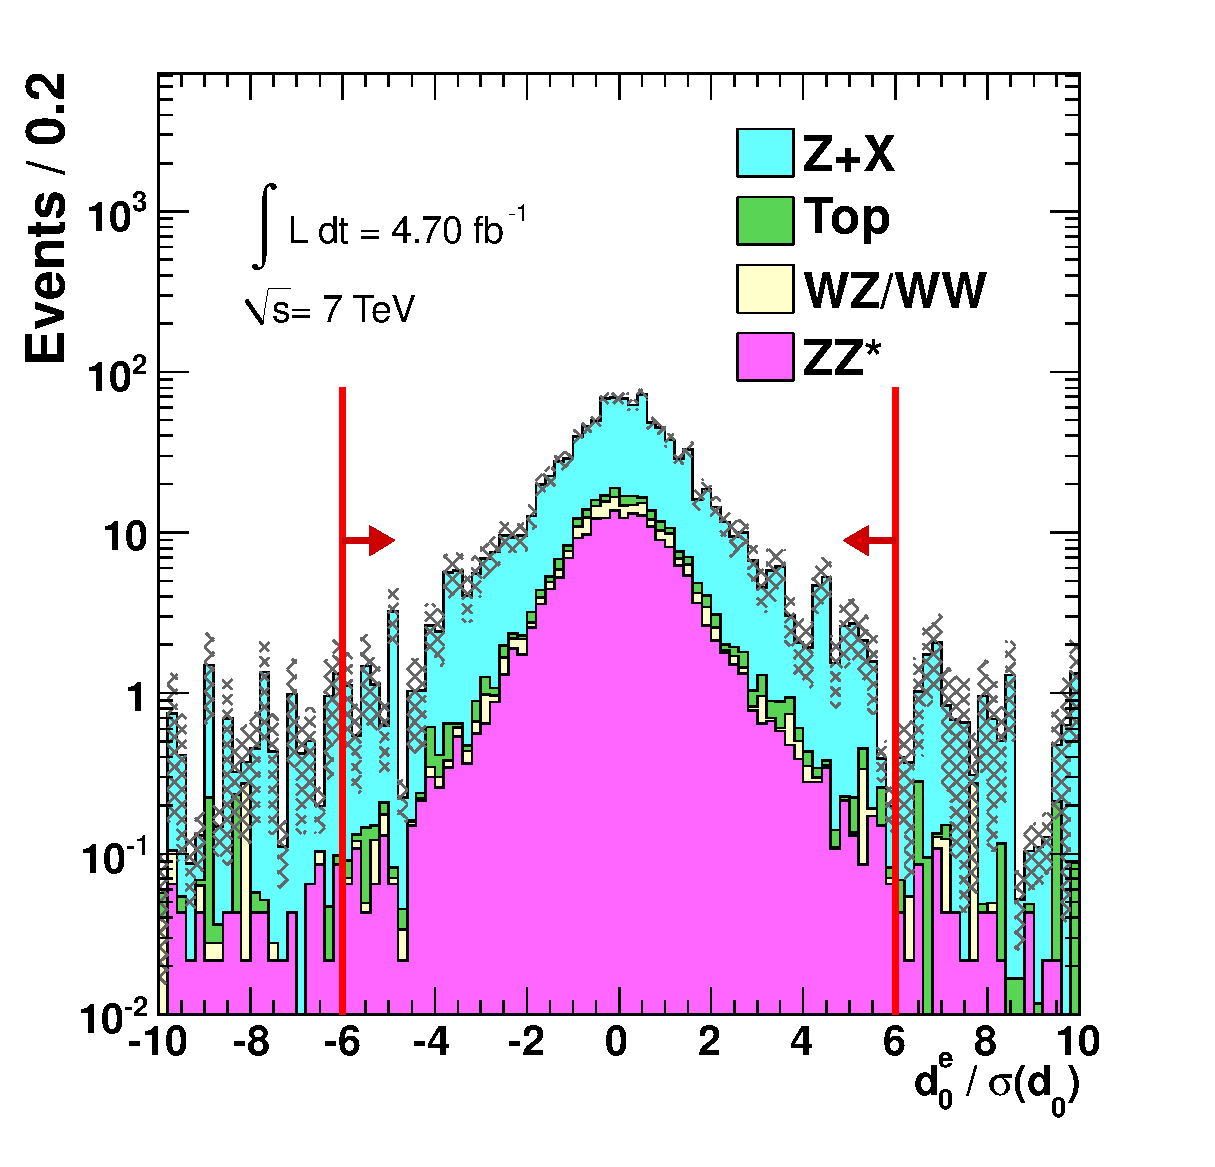
\includegraphics[width=0.47\textwidth]{ObjSel/h_4l_Electron_d0Sig_log}
        }
\caption[ ]{}
\label{fig:objsel-el}
\end{figure}

\section{Muon Selection}
\label{sec:objsel-mu}

\begin{table}[]
  \centering
%   \vspace*{-1cm}
\small
  \begin{tabular}{ l  l l }
    \hline\hline 
      Requirement        & 7 \tev\ & 8 \tev\ \\ 
      \hline
      \bf{Central Muons} & \\
      Algorithm             & \staco                        & \same \\
      Type                  & Combined or Segment Tagged    & \same \\
      $\eta$                & $|\eta|<2.5$                  & \same \\
      $p_T$                 & $p_T > 7$ GeV                 & \same \\
      ID Track Quality      & & \\
       - B Layer Hits       & $\geq 1$                      & \same \\
       - Pixel Hits         & $\geq 2$                      &  $\geq 1$\\
       - SCT Hits           & $\geq 6$                      &  $\geq 5$\\
       - Silicon `Holes'    & $<3$                          & \same \\
       - TRT                & \multicolumn{1}{p{5cm}}{\raggedright
                                {\bf If \modetalt{1.9}:} 
                                Require $n_{hits}+n_{outliers}>5$ 
                                and $n_{outliers}/(n_{hits}+n_{outliers})<0.9$}
                                                            & \multicolumn{1}{p{5cm}}{\raggedright
                                                                {\bf If \modetabetween{0.1}{1.9}:} 
                                                                Require $n_{hits}+n_{outliers}>5$ 
                                                                and $n_{outliers}/(n_{hits}+n_{outliers})<0.9$} \\
                            & \multicolumn{1}{p{5cm}}{\raggedright
                                {\bf If \modetagt{1.9}:} 
                                If $n_{hits}+n_{outliers}>5$ 
                                require $n_{outliers}/(n_{hits}+n_{outliers})<0.9$} 
                                                            & \multicolumn{1}{p{5cm}}{\raggedright
                                                                {\bf If \modetagt{1.9} or \modetalt{0.1}:} 
                                                                If $n_{hits}+n_{outliers}>5$ 
                                                                require $n_{outliers}/(n_{hits}+n_{outliers})<0.9$} \\
      \zzero                & $|z_0| < 2$ mm & $|z_0\sin(\theta)| < 0.5$ mm \\
      \dzerosig             & $|d_0|/\sigma(d_0) < 3.5 $    & \same \\
      Track isolation       & \ptconetwentylt{0.15}         & \same   \\
      Calorimeter isolation & \etconetwentylt{0.3}          & \it{Not Applied} \\
      \hline
      \bf{Forward Muons} & \\
      Algorithm             & \staco                        & \same \\
      Type                  & Combined or Stand-Alone       & \same \\
      $\eta$                & \modetabetween{2.5}{2.7}      & \same \\
      $p_T$                 & $p_T > 10$ GeV                & \same \\
      Calorimeter isolation & \etconetwentylt{0.15}         & \same \\
      % This is a cut that is automatically satisfied by combined
      %MS Track Quality      & Hits in all 3 stations       & \same \\
       \multicolumn{3}{c}{\it \underline{Additional requirements for Combined Muons}} \\
      ID Track Quality      &                               &  \\
       - B Layer Hits       & $\geq 1$                      & \same \\
       - Pixel Hits         & $\geq 2$                      & $\geq 1$\\
       - SCT Hits           & $\geq 4$                      & $\geq 3$\\
       - Silicon `Holes'    & $<3$                          & \same \\
      \zzero                & $|z_0| < 2$ mm                & $|z_0\sin(\theta)| < 0.5$ mm \\
      \dzerosig             & $|d_0|/\sigma(d_0) < 3.5 $    & \same \\
      \hline
      \multicolumn{2}{l}{\bf Calorimeter Tagged Muons} & \\
      Type                  & Calorimeter Tagged            & \same \\
      $\eta$                & \modetalt{0.1}                  & \same \\
      $p_T$                 & $p_T > 20$ GeV                & \same \\
      Quality               & Calorimeter Muon ID Cuts      & \same \\
      % This is a cut that is automatically satisfied by combined
      %MS Track Quality      & Hits in all 3 stations       & \same \\
      Overlap removal       & \multicolumn{1}{p{5cm}}{Remove 
                              if overlaps with a central 
                              muon in \deltaRlt{0.1}}  & \it{Same}\\
      \multicolumn{3}{c}{\it ID Track Quality, Track Isolation, Calorimeter
                                Isolation, \zzero, \dzerosig\ as central muons} \\
      %ID Track Quality      & As Central Muons              &  \\
      %Calorimeter isolation & \etconetwentylt{0.3}         & \same \\
      %Track isolation       & \ptconetwentylt{0.15}         & \same   \\
      %$z_0$                 & $|z_0| < 2$ mm                & $|z_0\sin(\theta)| < 0.5$ mm \\
      %$d_0$                 & $|d_0|/\sigma(d_0) < 3.5 $    & \same \\
                                                            
%
      %\bf{Central Electron Selection} & \\
      %Algorthim             & Standard (with GSF refit)     & Standard \\
      %Quality               & \multicolumn{2}{c}{\texttt{(OQ  AND 1446 == 0})} \\
      %ID cut                & \multicolumn{2}{c}{\loosePP}       \\
      %$\eta$                & \multicolumn{2}{c}{$|\eta|<2.47$} \\
      %$E_T$                 & \multicolumn{2}{c}{$E_T > 7$ GeV} \\
      %$z_0$                 & \multicolumn{2}{c}{$z_0 < 2$ mm} \\
      %$d_0$                 & \multicolumn{2}{c}{$|d_0|/\sigma(d_0) < 6 $} \\
      %Track isolation       & \multicolumn{2}{c}{\ptconetwentylt{0.15}}   \\
      %Calorimeter isolation & \etconetwentylt{0.3}          & \it{Not Applied} \\
      %Overlap removal       & \multicolumn{2}{c}{a) Remove $e$ if $\Delta R < 0.1$ from $\mu$} \\
      %                      & \multicolumn{2}{c}{b) Remove lowest $E_T$ $e$ in \deltaRlt{0.1} from another $e$} \\ 
      %\hline
      %\bf{Forward Electron Selection:} & \\
      %Alogirthm             & \multicolumn{2}{c}{Forward} \\
      %Quality               & \multicolumn{2}{c}{\texttt{(OQ  AND 1446 == 0)}}  \\
      %ID cut                & \multicolumn{2}{c}{Tight} \\
      %$\eta$                & \multicolumn{2}{c}{$2.50<|\eta|<3.16$} \\
      %$E_T$                 & \multicolumn{2}{c}{$E_T > 20$ GeV} \\
      %Overlap removal       & \multicolumn{2}{p{8cm}}{\centering Remove if overlaps with central electron or any muon in \deltaRlt{0.1}} \\
    \hline \hline
  \end{tabular}
   \caption{Muon selection requirements.}
   \label{table:objsel-mu}
\end{table}

Muon reconstruction was described in~\sec{reco-mu}. Three distinct categories of
muons are used in this analysis: `central' muons with \modetalt{2.5} and
`forward' muons with \modetabetween{2.5}{2.7}, both reconstructed with the
\staco\ algorithm, and calorimeter tagged muons with \modetalt{0.1},
reconstructed without using the muon spectrometer. As for electrons, additional
selection requirements are imposed to select muons likely to have originated from
\Z\ boson decays and to reject backgrounds. The muon selection requirements are
summarised in~\tab{objsel-mu} are described in more detail below. 

\subsection{Central Muon Selection}

Central muons must be either Combined (with a full MS and ID track) or Segment
Tagged (with a full ID track but only an MS track segment), and have $\pt>7$ GeV
and \modetalt{2.47}.

As for electrons, track and calorimeter isolation requirements are imposed to
reject backgrounds. In the case of muons this is mainly from heavy flavour
decays in jets and `punch-through' of hadrons into the muon spectrometer.  The
track isolation is defined in the same way as for electrons, and as for
electrons the requirement
is \ptconetwentylt{0.15}.  The calorimeter isolation variable is defined in a
similar way as for electrons, however the size of the `core' deposit of energy
attributed to the muon is smaller than in the case of electron isolation, and
varies by calorimeter component depending on the expected muon energy deposition
pattern (e.g. a single cell in the EM pre-sampler and 3x3 grid of cells in the second
layer of the EM calorimeter). The calorimeter isolation requirement is
\etconetwentylt{0.3}, and as for electrons is only applied to the 2011 data.

To ensure that the candidates come from the primary vertex, the magnitude
of the longitudinal impact parameter with respect to the primary vertex,
$|z_0|$ must be less than 2 mm for data taken in 2011. For data taken in 2012,
the requirement is $|z_0\sin(\theta)|<0.5$ mm. The transverse impact parameter
significance, \dzerosig is required to be less than 3.5. The selection for
muons is tighter than for electrons since because muons do not emit \brem\ to
the same extent as electrons the track fit is improved, and so the resolution of
the impact parameter is improved, so tighter requirements 
can be made whilst maintaining high signal efficiency.

The inner detector tracks associated with central muons must have a minimum
number of hits in each silicon sub-detector to ensure good track quality. For
2011 data the requirements are: at least 1 hit in the B-layer, $2$ in all Pixel
layers, $6$ in the SCT, and less than 3 holes (no hit in a layer crossed by the
track) in all silicon layers. For all silicon hit conditions, dead sensors count
as hits observed, not as holes.  Finally, a pseudo-rapidity dependent condition
on TRT hits and outliers is applied to ensure that the TRT extension of the
track is successful within the $\eta$ acceptance of the TRT (TRT hits can be
associated as outliers when the extension is not successful): for $|\eta| <
1.9$, require $\mathrm{hits}+\mathrm{outliers} > 6$ and $\mathrm{outliers} < 0.9
\times (\mathrm{outliers}+\mathrm{hits})$; for $|\eta| > 1.9$, if
$\mathrm{hits}+\mathrm{outliers} > 6$, require $\mathrm{outliers} < 0.9 \times
(\mathrm{outliers}+\mathrm{hits})$. For data taken in 2012, the
requirements are slightly loosened in order to recover efficiency losses in 2012
data; this was not found to increase the misidentification rate significantly;
see~\tab{objsel-mu} for details of the changes.

\subsection{Forward Muon Selection}

Muons in the region \modetabetween{2.5}{2.7} are required to have a full muon
spectrometer track with hits in each station of the spectrometer and have
\ptgt{10}. Although the
inner detector only extends to \modetaeq{2.5}, the complicated nature of the
magnetic field makes it possible for some muons up to \modetalt{2.6} to be
combined with an ID track, forming `Combined' muons; those that do not have an
ID track are termed Stand Alone.  In data reconstructed in 2012 muons without a
full ID track may be combined with pixel detector `tracklets' up to
\modetalt{2.65}. Such `Silicon Associated' muons benefit from improved vertex
parameter estimation, but are otherwise treated as Stand Alone. 

Since not all forward muons
have tracks, a track isolation requirement is not applied; instead a tighter calorimeter isolation
requirement is applied to forward muons: \etconetwentylt{0.15}. This is applied
to both 2011 and 2012 data.

For forward muons with an ID track, a set of ID track quality
cuts are applied to the number of hits in the silicon detectors, similar to the
cuts for central muons but slightly looser. For data taken in 2011
the requirements are: at least 1 hit in the B-layer, $2$ in all Pixel layers,
$4$ in the SCT, and less than 3 holes (no hit in a layer crossed by the track)
in all silicon layers. No cut is applied to the number of TRT hits. As for
central muons, the requirements were relaxed slightly for 2012 data.
Additionally, forward muons with an ID track are required to satisfy the same
\zzero\ and \dzerosig\ requirements as central muons.

\subsection{Calorimeter Tagged Muon Selection}

Calorimeter tagged muons are used to recover efficiency at \modetalt{0.1} where
there is a gap in the muon-spectrometer. They must have \ptgt{20}. The reason
for this higher \pt\ requirement is the higher level of fakes from jets and
electrons at low \pt, and the difficulty of measuring the identification
efficiency for $\pt<20\gev$. They are required to pass either the cut or
likelihood based calorimeter tagged muon identification requirements described
in~\sec{reco-mu-reco}, and are not selected if they overlap with a selected
central muon within \deltaRlt{0.1}. Calorimeter tagged muons must satisfy the
same track and calorimeter isolation, ID track quality, \zzero\ and \dzerosig\
requirements as central muons.

\begin{figure}[h]
\centering
	\subfigure[]{
            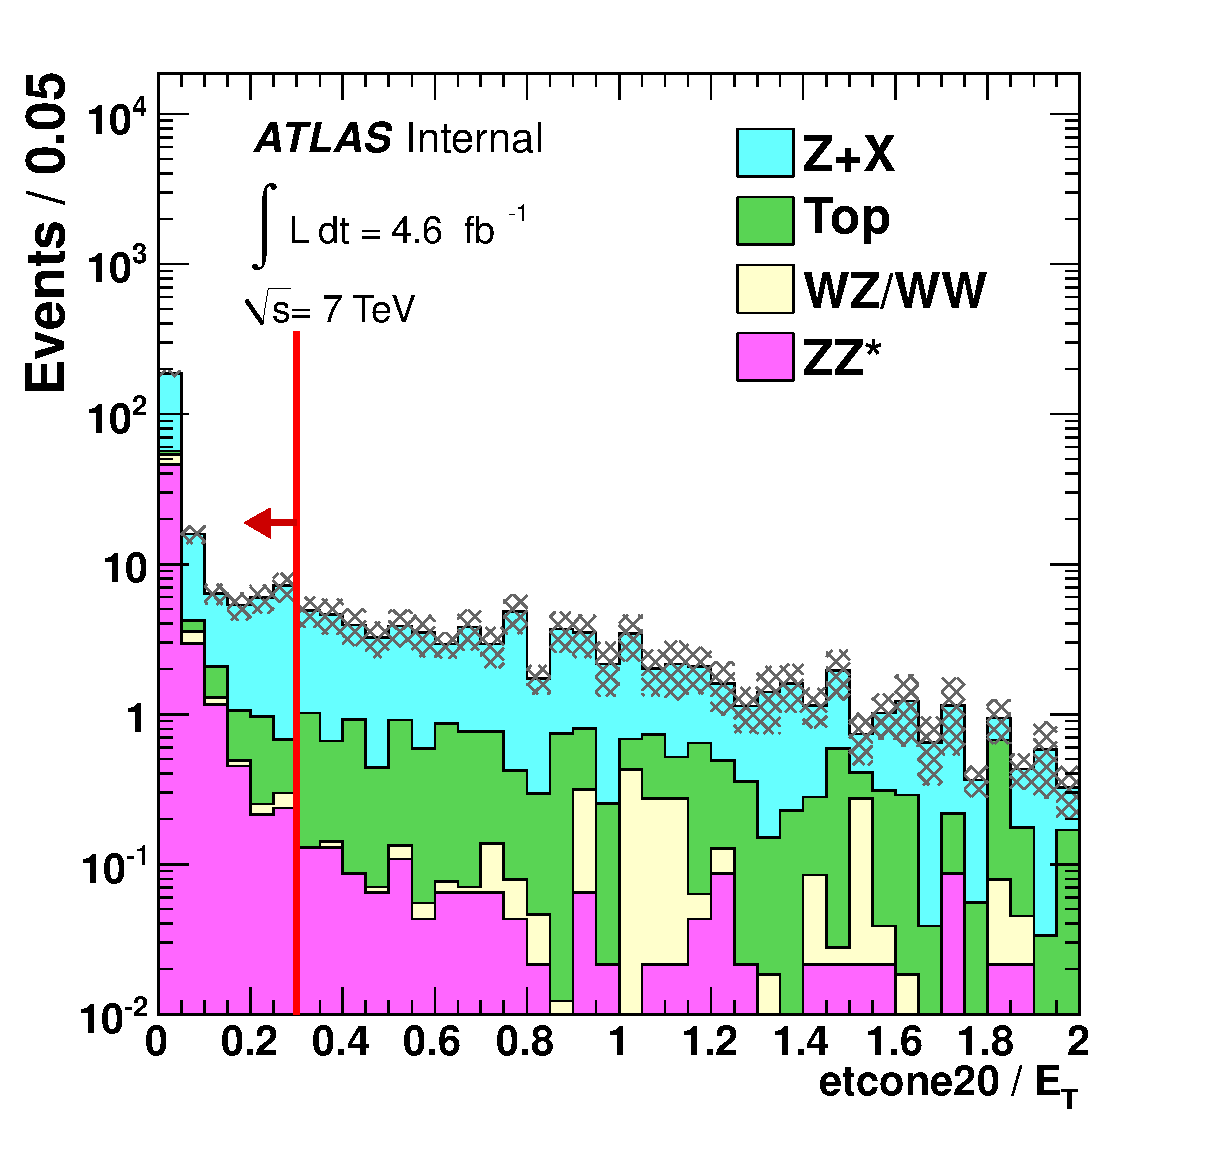
\includegraphics[width=0.47\textwidth]{ObjSel/h_4l_MuEtCone20_log}
        }
	\subfigure[]{
            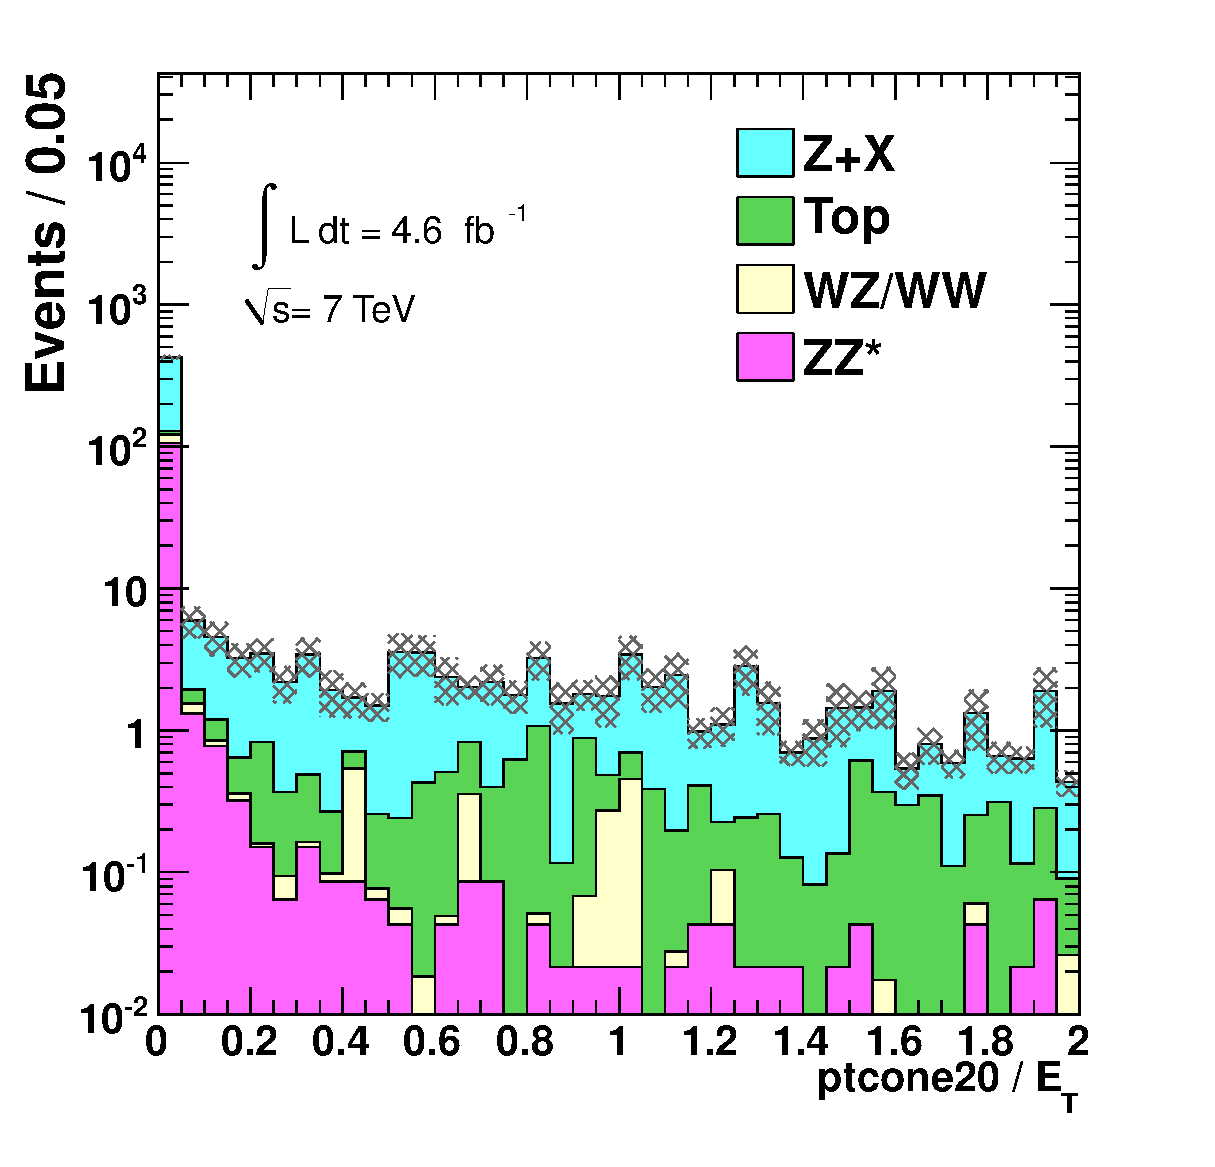
\includegraphics[width=0.47\textwidth]{ObjSel/h_4l_MuPtCone20_log}
        }
	\subfigure[]{
            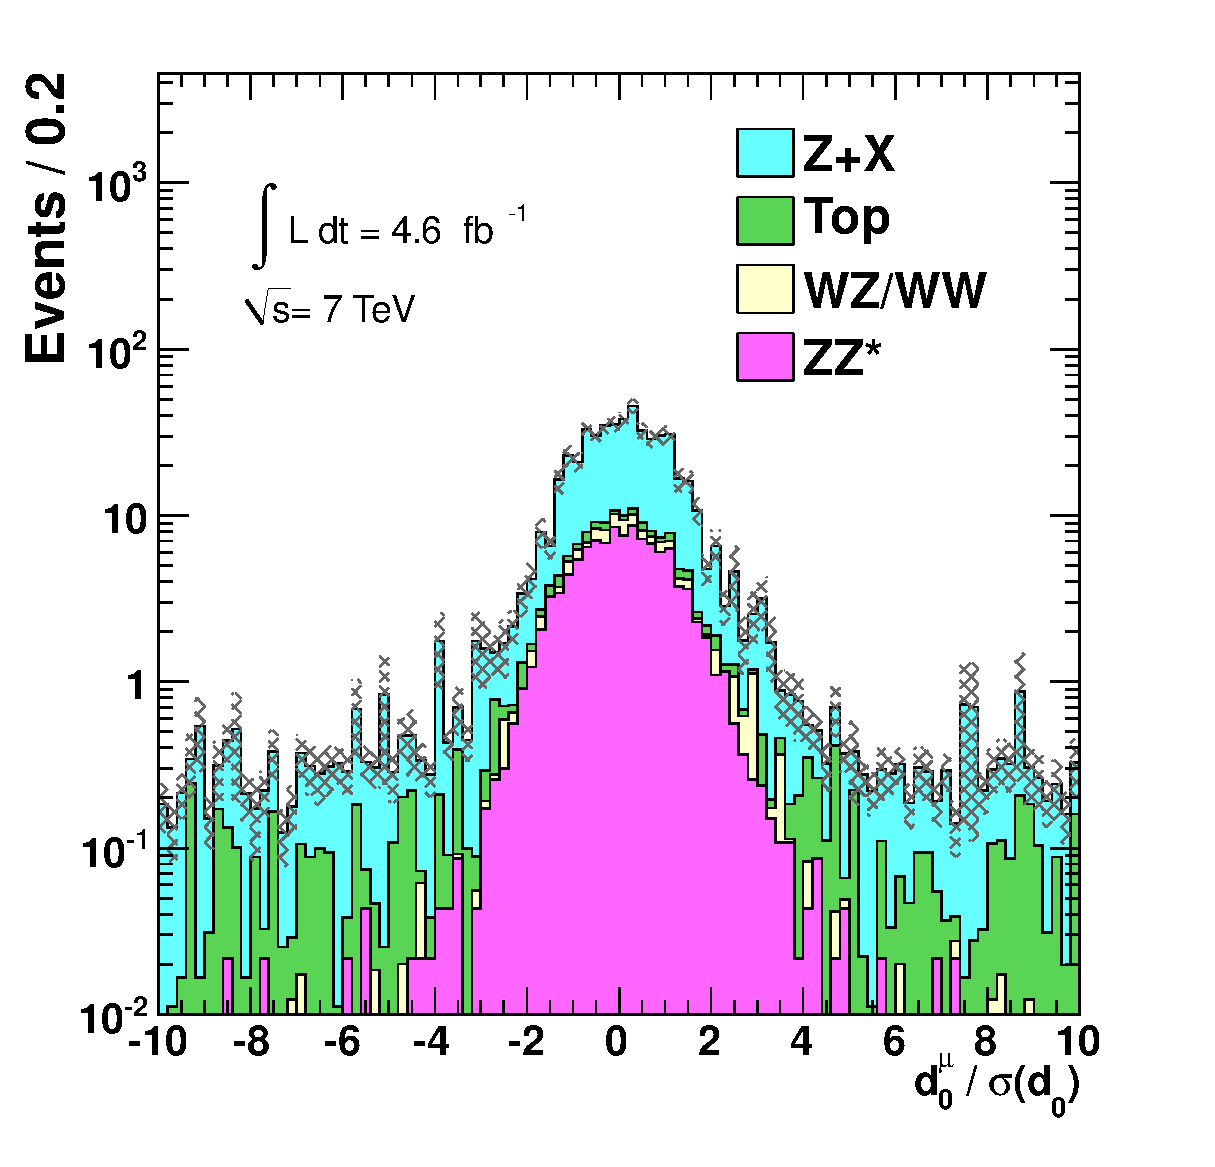
\includegraphics[width=0.47\textwidth]{ObjSel/h_4l_Muon_d0Sig_log}
        }
\caption[ ]{}
\label{fig:objsel-mu}
\end{figure}

%\section{Jet Selection}

\section{Triggers}
\label{sec:triggers}

\ZZ\ candidate events in are triggered using the lowest threshold unprescaled single-electron or
single-muon triggers, as descried in Section~\ref{sec:reco-el-triggers}
and~\ref{sec:reco-mu-triggers}. For the \eemm\ final state, the event may be selected using either
the electron trigger or the single muon trigger. The triggers used in the
different data taking periods and the
associated luminosity are shown in~\tab{objSel-trigger-el} for the electron
trigger and~\tab{objSel-trigger-mu} for the muon trigger.

\begin{table}[htbp]
\begin{center}
%\small
\begin{tabular}{lccc p{5cm}}
\hline \hline
Period & Trigger & \pt\ Threshold (GeV) & Int. Luminosity (\ifb) \\
\hline
{ \bf 2011 } & & & \\
B - I & \texttt{e20\_medium} & 20 &  1.65 \\
J - K & \texttt{e22\_medium} & 22 & 0.91 \\
L - M & \texttt{e22vh\_medium1} & 22 & 2.76 \\ \hline
%L - M & \texttt{e22vh\_medium1} & 22 & 2.76 & Variable L1 thresholds; hadronic leakage requirement \\ \hline
\hline
{ \bf 2012 } & & & \\
A - M & \multicolumn{1}{p{4cm}}{\centering \texttt{e24vhi\_medium1} $||$ \texttt{e60\_medium1}} & 24 & \LumiTotalReadyTwentyTwelve \\
\hline\hline
\end{tabular}
\end{center}
\caption{Electron triggers used in the different data taking periods.}
\label{table:objSel-trigger-el}
\end{table}

\begin{table}[htbp]
\begin{center}
%\small
\begin{tabular}{lccc p{5cm}}
\hline \hline
Period & Trigger & \pt\ Threshold (GeV) & Int. Luminosity (\ifb) \\
\hline
{ \bf 2011 } & & & \\
B - I & \texttt{mu18\_MG} & 18 &  1.65 \\
J - M & \texttt{mu18\_MG\_medium} & 18 & 3.67 \\
%L - M & \texttt{e22vh\_medium1} & 22 & 2.76 & Variable L1 thresholds; hadronic leakage requirement \\ \hline
\hline
{ \bf 2012 } & & & \\
A - M & \multicolumn{1}{p{4cm}}{\centering \texttt{mu24i\_tight} $||$ \texttt{mu36\_tight}} & 24 & \LumiTotalReadyTwentyTwelve \\
\hline\hline
\end{tabular}
\end{center}
\caption{Muon triggers used in the different data taking periods.}
\label{table:objSel-trigger-mu}
\end{table}

At least one selected lepton in triggered events must match to the
object that caused the trigger to fire. Such leptons are referred to as 
\intro{trigger matched} leptons. To reduce uncertainties associated with the
trigger efficiency measurement, to be considered trigger matched
a lepton must have a \pt\ such that it is on the efficiency plateau of the
trigger, and must also satisfy the same identification requirements as
used in the trigger. Trigger matched leptons in both 2011 and 2012 data
are required to have \ptgt{25}, cluster \modetalt{2.47} and to pass the \mediumPP\
requirements. Trigger matched muons are required to be combined muons, have
\modetalt{2.4} and have $\pt > 20 (25)$ \gev\ in 2011 (2012) data.

The efficiency for a single lepton to fire the trigger is measured in data using
\Zll\ events. Events are triggered on by a `tag' lepton, then the efficiency for
the second `probe' lepton to fire the trigger is measured. By comparing the
efficiencies in data and in \mc\ simulation, scale-factors are derived to
correct the single lepton trigger efficiencies in the simulation to that
observed in data. 
This is translated to an event level trigger efficiency
scale-factor using the following formula:

\begin{equation}
\label{eq:triggerEffSF}
  SF =  { \frac{ {1 - \prod_{n=1}^{N_l} (1 - \epsilon_{Data,l_n})}} {1 - \prod_{n=1}^{N_l} (1 - \epsilon_{MC,l_n})} }
\end{equation}

where $N_l$ is the number of leptons passing the trigger matching kinematic and
identification requirements
given above (but not necessarily trigger matched),
$\epsilon_{Data,l_n}$ is the trigger efficiency in data, determined as above,
for a lepton of flavour flavor $l_n$, and $\epsilon_{MC,l_n}$ is
the corresponding efficiency determined in the MC. 
%The systematic uncertainty associated with the scale factors for
%muon triggers is $0.2\%$ and for electron triggers is $\sim1\%$. 

Trigger efficiencies for \ZZ\ events passing the full event selection
described below, derived from simulation after applying the scale-factors
described above, are listed in~\tab{triggerMCeff}.

\begin{table}[htbp]
\begin{center}
\renewcommand\arraystretch{1.12}
\begin{tabular}{ccc}
\hline \hline
Channel & \multicolumn{2}{c}{Trigger Efficiency [\%]} \\
\hline
      & \ZZ\ Selection     & \ZZs\ Selection      \\
%Channel & Trigger Efficiency [\%] & Shift when applying SF [\%]\\
%
\hline
                   $eeee$ & 100.0$^{+0.0}_{-0.4}$   & 99.6$^{+0.2}_{-0.5}$ \\
           $\mu\mu\mu\mu$ & 98.7$^{+0.4}_{-0.6}$    & 98.2$^{+0.4}_{-0.5}$ \\
               $ee\mu\mu$ & 99.6$^{+0.2}_{-0.3}$    & 98.8$^{+0.3}_{-0.4}$ \\
                   $llll$ & 99.4$^{+0.2}_{-0.2}$    & 98.8$^{+0.2}_{-0.2}$ \\
    \hline \hline
\end{tabular}
\defaultArrayStretch
\end{center}
\caption{Trigger efficiencies for \ZZ\ events after all selection cuts excluding the trigger match and trigger requirement.
Scale-factors are applied on a per-object basis to reproduce the trigger efficiency measured in data in the Monte-Carlo.
}
\label{table:triggerMCeff}
\end{table}

\section{Dilepton Control Plots}

\section{\ZZ\ Event Selection}
\label{sec:eventsel}

\subsection{\Z\ Candidate Definitions}

In referring to \Z\ candidate \dilep\ pairs, the following definitions are used:

\begin{itemize}

    \item {\bf Leading and Subleading:} The \Z\ candidate with the greatest \pt\
    of the pair is referred to as the \intro{leading} \Z; the \Z\ candidate with the
    lower \pt\ is referred to as the \intro{subleading} \Z.

    \item {\bf Primary and Secondary:} The \Z\ candidate closest to the \Z\
    boson mass (from~\cite{PDG}) is referred to as the \intro{primary} \Z; the other
    candidate is referred to as the \intro{secondary} \Z.

\end{itemize}

There is a strong correlation between the \pt\ of a \Z\ candidate and its distance
from the \Z\ mass, as seen in~\figs{data-zmass-zpt-seven}{data-zmass-zpt-eight},
so it is often, but not always, the case that the leading \Z\ candidate is also the primary
\Z\ candidate.

\subsection{Event Selection Requirements}

Candidate \ZZ\ events are selected using the following requirements:

\begin{enumerate}

    \item {\bf Data Quality Requirements:} Events are required to pass a `Good
    Run List' to remove events occurring in a Lumiblock where there were defects
    affecting the quality of the data, for example a ROD (Read Out Device) going `busy' meaning
    data from a large fraction of a subdetector was missing.

    \item {\bf Trigger:} The event must pass a high \pt\ single electron or single
    muon trigger as discussed in~\sec{triggers}.

    \item {\bf Four leptons:} The event must have exactly four electrons or muons
    passing the selection requirements described in Sections~\ref{sec:objsel-el}
    and~\ref{sec:objsel-mu}. This cut simplifies the equations for the background
    estimate. MC predictions show that 1.3\% of signal events would fail this cut. In
    data, no events with more than four fully selected leptons were observed.

    \item {\bf Lepton Separation:} The leptons are required to be spatially separated by
    $\Delta{R}(\ell,\ell)>0.2$. This requirement is automatically satisfied by
    the lepton isolation requirements applied to all leptons except forward
    electrons. It is made here explicitly since it is important in the
    background estimate(~see \chap{bg}), and to highlight the fact that there is no
    analysis sensitivity to events with leptons separated by \deltaRlt{0.2},
    which is of importance when performing searches for nTGCs, where the \Z\
    bosons are expected to be heavily boosted and this the leptons close
    together in the detector frame. This is discussed in more detail below.

    \item {\bf Trigger match:} At least one selected lepton must match to the
    object that caused the trigger to fire, as described above. 

    \item {\bf Quadruplet Formation:} There must be two same flavour,
    oppositely charged lepton pairs. In $eeee$ and $\mu\mu\mu\mu$ events there are
    two possible ways of pairing the four leptons into OS pairs. The pairing which
    minimises the quantity $|m_{12}-m_{Z}|+|m_{34}-m_{Z}|$ is chosen, where
    $m_{12}$, $m_{34}$ are the invariant masses of the two lepton pairs of a certain
    pairing of the lepton quad consisting of leptons '1','2','3','4' and $m_Z$ is
    the \Z\ boson mass, taken from~\cite{PDG}.

    \item {\bf ``Primary" \Z\ candidate:} The primary \Z\ candidate must satisfy the mass cut $66<m_{12}<116$~GeV.

    \item {\bf ``Secondary" \Z\ candidate} Two non-exclusive mass cuts are
    applied to the secondary \Z\ candidate, one
    to select the event as a \ZZ\ event, the other to select the event as a
    \ZZs\ event:
      \begin{enumerate}
     \item To be classified as a \ZZ\ event the secondary \Z\ candidate must satisfy
     the mass cut $66<m_{34}<116$~GeV.
     \item To be classified as a \ZZs\ event the secondary \Z\ candidate
     must satisfy the mass cut $m_{34}>20$~GeV.
    \end{enumerate}

\end{enumerate}

Applying these requirements, a total
of~\ZZSevenTeVNSigEventsObsZZLLLL\ (\ZZSevenTeVNSigEventsObsZZsLLLL) events
are observed in the 2011 data for the \ZZ\ (\ZZs) selection. In the 2012 data, 
~\ZZEightTeVNSigEventsObsZZLLLL\ (\ZZEightTeVNSigEventsObsZZsLLLL) events are
observed for the \ZZ\ (\ZZs) selection. The expected number of events in
\LumiPassGRLTwentyEleven\ \ifb\ of 7~\tev\ data after various stages of the
selection is shown in~\tab{objSel-cutflow-seven}. The corresponding numbers for
\LumiPassGRLTwentyTwelve\ \ifb\ of 8~\tev\ data are shown
in~\tab{objSel-cutflow-eight}.

%%%%%%%%%%%%%%%%%%%%%%%%%%%%%
% Updated to 4.6fb-1 numbers for paper
% Nick, 25/5/2012
% No fwdEIso, fwd e, mu SF
%%%%%%%%%%%%%%%%%%%%%%%%%%%%%
\begin{table}[htbp]
	 \centering
         \small
	 \begin{tabular}{lcccc}
	 \hline\hline
%	 	 Cutflow & \multicolumn{4}{|c|}{Number of Events} \\ \cline{2-5}
$N_{ZZ}$ (7~\tev, \LumiPassGRLTwentyEleven\ \ifb)	  & \llll\  & \eeee\ & \mmmm\ & \eemm\ \\
	 	 \hline
   Four leptons             &  82.27 $\pm$ 0.43  &  15.23 $\pm$ 0.17 &  25.49 $\pm$ 0.23  &  41.55 $\pm$ 0.31 \\ 
   Trigger Match            &  80.66 $\pm$ 0.41  &  15.01 $\pm$ 0.17 &  24.93 $\pm$ 0.23  &  40.69 $\pm$ 0.31  \\ 
   Quadruplet               &  79.41 $\pm$ 0.41  &  14.51 $\pm$ 0.17 &  24.92 $\pm$ 0.23  &  39.98 $\pm$ 0.29  \\ 
   Primary Z mass           &  69.21 $\pm$ 0.38  &  12.92 $\pm$ 0.16 &  21.60 $\pm$ 0.22  &  34.67 $\pm$ 0.28  \\ 
   Secondary Z mass, \ZZs   &  65.37 $\pm$ 0.37  &  12.51 $\pm$ 0.15 &  20.35 $\pm$ 0.21  &  32.50 $\pm$ 0.27  \\ 
   Secondary Z mass, ZZ     &  53.41 $\pm$ 0.34  &  10.28 $\pm$ 0.14 &  16.45 $\pm$ 0.19  &  26.67 $\pm$ 0.24  \\

	 \hline\hline
	 \end{tabular}
           \caption{Expected number of events in 7~\tev\ data by cut for
           $\mathcal{L}=4.6 {\rm fb}^{-1}$. The errors are statistical only. The
           contribution from $\ZZ \to \tau+X$ where the tau decays into an
           electron or a muon is included; the estimated contribution is given
           in~\tab{objSel-czz-seven}.}
          \label{table:objSel-cutflow-seven}
\end{table}

\begin{table}[htbp]
	 \centering
         \small
	 \begin{tabular}{lcccc}
	 \hline\hline
%	 	 Cutflow & \multicolumn{4}{|c|}{Number of Events} \\ \cline{2-5}
$N_{ZZ}$ (8~\tev, \LumiPassGRLTwentyTwelve\ \ifb)	  & \llll\  & \eeee\ & \mmmm\ & \eemm\ \\
	 	 \hline
   Four leptons             &  xx.xx $\pm$ x.xx  &  xx.xx $\pm$ x.xx &  xx.xx $\pm$ x.xx  &  xx.xx $\pm$ x.xx \\ 
   Trigger Match            &  xx.xx $\pm$ x.xx  &  xx.xx $\pm$ x.xx &  xx.xx $\pm$ x.xx  &  xx.xx $\pm$ x.xx  \\ 
   Quadruplet               &  xx.xx $\pm$ x.xx  &  xx.xx $\pm$ x.xx &  xx.xx $\pm$ x.xx  &  xx.xx $\pm$ x.xx  \\ 
   Primary Z mass           &  xx.xx $\pm$ x.xx  &  xx.xx $\pm$ x.xx &  xx.xx $\pm$ x.xx  &  xx.xx $\pm$ x.xx  \\ 
   Secondary Z mass, \ZZs   &  xx.xx $\pm$ x.xx  &  xx.xx $\pm$ x.xx &  xx.xx $\pm$ x.xx  &  xx.xx $\pm$ x.xx  \\ 
   Secondary Z mass, ZZ     &  xx.xx $\pm$ x.xx  &  xx.xx $\pm$ x.xx &  xx.xx $\pm$ x.xx  &  xx.xx $\pm$ x.xx  \\

	 \hline\hline
	 \end{tabular}
           \caption{Expected number of events in 8~\tev\ data by cut for
           $\mathcal{L}=4.6 {\rm fb}^{-1}$. The errors are statistical only. The
           contribution from $\ZZ \to \tau+X$ where the tau decays into an
           electron or a muon is included; the estimated contribution is given
           in~\tab{objSel-czz-eight}.}
          \label{table:objSel-cutflow-eight}
\end{table}

\section{Selection Efficiencies}

\subsection{Reconstruction Acceptance \CZZ}

In order to extrapolate from the number of observed events to a \cx\ or similar
measurement, it is necessary to know the acceptance of the selection
requirements. This is described by the \intro{reconstruction acceptance factor,
\CZZ}. Formally, this is defined as:

\begin{equation}
C_{ZZ}= \epsilon_{trig} \times \epsilon_{event} \times \epsilon_{lep} \times \alpha_{reco}
\end{equation}

where $\epsilon_{trig}$ is the trigger efficiency, $\epsilon_{event}$ is 
the efficiency of the event level cuts, and
$\epsilon_{lep} =\epsilon_{lep1}\epsilon_{lep2}\epsilon_{lep3}\epsilon_{lep4}$ is the product of the 
individual reconstruction and selection efficiencies for the four leptons. 
$\alpha_{reco}$ is the reconstruction to 
fiducial phase space correction which corrects for small differences between the
regions of phase space covered by detector acceptance and the definition of the
fiducial phase space; it also accounts for effects of detector resolution. 

In practice, \CZZ\ is estimated from \mc\ by dividing the number of events in a
\ZZllll\ sample which pass the selection requirements by the number of those events
which were generated inside the fiducial phase space. This is shown in the
following equation:

\begin{equation}
C_{ZZ}= \frac{ N^{\rm MC\ Pass\ All\ Cuts}_{{\rm Reconstructed}\ ZZ} \times
SF }{ N^{{\rm MC\ Fiducial\ Volume}}_{{\rm Generated}\ ZZ} }
\end{equation}

where {\it SF} is the event level scale factor applied to the \mc\ to correct
lepton selection efficiencies and trigger efficiencies to those observed in
data. The number in the denominator includes contributions from
$\ZZ\ra\tau\tau\ell\ell$ decays (and to a smaller extent
$\ZZ\ra\tau\tau\tau\tau$), where the taus decay leptonically. The numerator also
includes a contribution from events generated outside the fiducial volume but
which are reconstructed as within, for example an event with a generated lepton
with a \pt\ just lower than the lepton \pt\ threshold which is reconstructed
with an energy just above the threshold. Since the numerator is not a subset of
the denominator due to these two contributions, \CZZ\ is not a true efficiency. 

\CZZ\ is calculated separately for each of the three final states (\eeee, \mmmm\
and \eemm), and separately for the \ZZ\ and \ZZs\ selection and for the 7 \tev\
and 8 \tev\ analysis. Values for \CZZ\ are given
in~\tabs{objSel-czz-seven}{objSel-czz-eight}, as well as the estimated
contribution from tau decays and events generated outside the fiducial volume.
Also given is the true selection efficiency, defined analogously to \CZZ, but
with only events generated in the fiducial phase space included in the numerator
such that the numerator is a subset of the denominator.

The reconstruction efficiency in the \eeee\ final state is significantly worse
than in the \mmmm\ final state: as much as to 40\% lower for the \ZZs\ selection
at 7~\tev. This is attributed to the lower reconstruction and identification
efficiencies for electrons compared to muons. Since in a \fourlep\ final state
the average event level selection efficiency is the fourth power of the average
single lepton selection efficiency, differences in efficiency between electrons
and muons get significantly simplified. The reconstruction efficiency is 
slightly lower for the \ZZs\ selection than for the \ZZ\ selection, particularly
in final states with electrons; as much as
6\% in the \eeee\ final state at 7~\tev. This can be attributed to the higher
proportion of leptons at low \pt\ in the \ZZs\ selection, and the fact that the
electron identification efficiency drops off significantly below
20~\gev\ (see~\fig{el-id-eff-et}).

The percentage of tau events passing the selection requirements is approximately
0.5\% for the \ZZ\ selection and $\sim2\%$ for the \ZZs\ selection. This higher
contamination in the \ZZs\ selection can be accounted for by the fact that
\dielectron\ or \dimuon\ pairs from decays of a di-tau pair with an invariant mass
near the \Z\ mass will have a lower invariant mass due to the energy carried
away by the neutrinos. There is therefore a higher chance of them passing the
looser mass cut applied in the \ZZs\ selection than passing the \sstooos\ mass
cut applied in the \ZZ\ selection. The contamination from events outside the
fiducial phase space is similar in the \ZZ\ and \ZZs\ selections, at a level of
$\sim1\%$.

% TODO
{\bf MAKE COMPARISONS OF CZZ IN 2011 AND 2012}

%The reconstruction efficiency is seen to 

\begin{table}[htbp]
\small
    \centering
    \begin{tabular}{p{3.5cm}llll}
    %\begin{tabular}{p{3cm}p{1.2cm}p{1.2cm}p{1.2cm}p{1.2cm}}
	\hline\hline
        \ZZ, 7~\tev & \eeee & \mmmm & \eemm & \llll \\
        \hline

        % C_ZZ
        \raggedright Reconstruction acceptance $C_{ZZ}$  & 
        \ZZSevenTeVCzzZZEEEE\ $\pm$  \ZZSevenTeVCzzStatZZEEEE &
        \ZZSevenTeVCzzZZMMMM\ $\pm$  \ZZSevenTeVCzzStatZZMMMM &
        \ZZSevenTeVCzzZZEEMM\ $\pm$  \ZZSevenTeVCzzStatZZEEMM &
        \ZZSevenTeVCzzZZLLLL\ $\pm$  \ZZSevenTeVCzzStatZZLLLL \\
        \hline

          \raggedright Contamination from $\ZZ\ra\tau+X$ (\%)  & 
        \ZZSevenTeVTauContaminationPercentageZZEEEE\ $\pm$  \ZZSevenTeVTauContaminationPercentageStatZZEEEE &
        \ZZSevenTeVTauContaminationPercentageZZMMMM\ $\pm$  \ZZSevenTeVTauContaminationPercentageStatZZMMMM &
        \ZZSevenTeVTauContaminationPercentageZZEEMM\ $\pm$  \ZZSevenTeVTauContaminationPercentageStatZZEEMM &
        \ZZSevenTeVTauContaminationPercentageZZLLLL\ $\pm$  \ZZSevenTeVTauContaminationPercentageStatZZLLLL \\
        \hline
        %%
         % Contaminations from outside fid
         \raggedright Contamination from events outside fiducial region(\%)   & 
        \ZZSevenTeVOutsideFidContaminationPercentageZZEEEE\ $\pm$  \ZZSevenTeVOutsideFidContaminationPercentageStatZZEEEE &
        \ZZSevenTeVOutsideFidContaminationPercentageZZMMMM\ $\pm$  \ZZSevenTeVOutsideFidContaminationPercentageStatZZMMMM &
        \ZZSevenTeVOutsideFidContaminationPercentageZZEEMM\ $\pm$  \ZZSevenTeVOutsideFidContaminationPercentageStatZZEEMM &
        \ZZSevenTeVOutsideFidContaminationPercentageZZLLLL\ $\pm$  \ZZSevenTeVOutsideFidContaminationPercentageStatZZLLLL \\
        \hline

        % "True" C_ZZ
        \raggedright True reconstruction efficiency      & 
        \ZZSevenTeVTrueCzzZZEEEE\ $\pm$  \ZZSevenTeVTrueCzzStatZZEEEE &
        \ZZSevenTeVTrueCzzZZMMMM\ $\pm$  \ZZSevenTeVTrueCzzStatZZMMMM &
        \ZZSevenTeVTrueCzzZZEEMM\ $\pm$  \ZZSevenTeVTrueCzzStatZZEEMM &
        \ZZSevenTeVTrueCzzZZLLLL\ $\pm$  \ZZSevenTeVTrueCzzStatZZLLLL \\

	\hline\hline
        \\

	\hline\hline
        \ZZs, 7~\tev & \eeee & \mmmm & \eemm & \llll \\
        \hline

        % C_ZZ
        \raggedright Reconstruction acceptance $C_{ZZ}$  & 
        \ZZSevenTeVCzzZZsEEEE\ $\pm$  \ZZSevenTeVCzzStatZZsEEEE &
        \ZZSevenTeVCzzZZsMMMM\ $\pm$  \ZZSevenTeVCzzStatZZsMMMM &
        \ZZSevenTeVCzzZZsEEMM\ $\pm$  \ZZSevenTeVCzzStatZZsEEMM &
        \ZZSevenTeVCzzZZsLLLL\ $\pm$  \ZZSevenTeVCzzStatZZsLLLL \\
        \hline

          \raggedright Contamination from $\ZZ\ra\tau+X$ (\%)  & 
        \ZZSevenTeVTauContaminationPercentageZZsEEEE\ $\pm$  \ZZSevenTeVTauContaminationPercentageStatZZsEEEE &
        \ZZSevenTeVTauContaminationPercentageZZsMMMM\ $\pm$  \ZZSevenTeVTauContaminationPercentageStatZZsMMMM &
        \ZZSevenTeVTauContaminationPercentageZZsEEMM\ $\pm$  \ZZSevenTeVTauContaminationPercentageStatZZsEEMM &
        \ZZSevenTeVTauContaminationPercentageZZsLLLL\ $\pm$  \ZZSevenTeVTauContaminationPercentageStatZZsLLLL \\
        \hline
        %%
         % Contaminations from outside fid
         \raggedright Contamination from events outside fiducial region(\%)   & 
        \ZZSevenTeVOutsideFidContaminationPercentageZZsEEEE\ $\pm$  \ZZSevenTeVOutsideFidContaminationPercentageStatZZsEEEE &
        \ZZSevenTeVOutsideFidContaminationPercentageZZsMMMM\ $\pm$  \ZZSevenTeVOutsideFidContaminationPercentageStatZZsMMMM &
        \ZZSevenTeVOutsideFidContaminationPercentageZZsEEMM\ $\pm$  \ZZSevenTeVOutsideFidContaminationPercentageStatZZsEEMM &
        \ZZSevenTeVOutsideFidContaminationPercentageZZsLLLL\ $\pm$  \ZZSevenTeVOutsideFidContaminationPercentageStatZZsLLLL \\
        \hline

        % "True" C_ZZ
        \raggedright True reconstruction efficiency      & 
        \ZZSevenTeVTrueCzzZZsEEEE\ $\pm$  \ZZSevenTeVTrueCzzStatZZsEEEE &
        \ZZSevenTeVTrueCzzZZsMMMM\ $\pm$  \ZZSevenTeVTrueCzzStatZZsMMMM &
        \ZZSevenTeVTrueCzzZZsEEMM\ $\pm$  \ZZSevenTeVTrueCzzStatZZsEEMM &
        \ZZSevenTeVTrueCzzZZsLLLL\ $\pm$  \ZZSevenTeVTrueCzzStatZZsLLLL \\

	\hline\hline
    \end{tabular}
    \caption{Details of the acceptance and selection
    efficiencies and contaminations, estimated from \mc, for the \ZZ\ and \ZZs\
    selections in the 7~\tev\ analysis. The first row shows the the
    reconstruction factor \CZZ\, defined as the ratio of the number of events
    passing the selection requirements (including contributions from $\ZZ
    \rightarrow \tau+X$ and events outside the fiducial region) to the number
    of generated events in the fiducial region.  The second row shows the
    percentage contamination from $\rightarrow \tau+X$ events, and the third
    the percentage contamination from events falling outside of the fiducial
    region at generator level, but passing the selection due to the energy,
    momentum or track direction being mis-reconstructed.  The final row shows
    the ``true'' reconstruction efficiency, with the contribution from $\ZZ
    \rightarrow \tau+X$ and events outside the fiducial region removed from the
    numerator.  All errors shown are statistical only.}
    \label{table:objSel-czz-seven}
\end{table}

\begin{table}[htbp]
\small
    \centering
    \begin{tabular}{p{3.5cm}llll}
    %\begin{tabular}{p{3cm}p{1.2cm}p{1.2cm}p{1.2cm}p{1.2cm}}
	\hline\hline
        \ZZ, 7~\tev & \eeee & \mmmm & \eemm & \llll \\
        \hline

        % C_ZZ
        \raggedright Reconstruction acceptance $C_{ZZ}$  & 
        \ZZEightTeVCzzZZEEEE\ $\pm$  \ZZEightTeVCzzStatZZEEEE &
        \ZZEightTeVCzzZZMMMM\ $\pm$  \ZZEightTeVCzzStatZZMMMM &
        \ZZEightTeVCzzZZEEMM\ $\pm$  \ZZEightTeVCzzStatZZEEMM &
        \ZZEightTeVCzzZZLLLL\ $\pm$  \ZZEightTeVCzzStatZZLLLL \\
        \hline

          \raggedright Contamination from $\ZZ\ra\tau+X$ (\%)  & 
        \ZZEightTeVTauContaminationPercentageZZEEEE\ $\pm$  \ZZEightTeVTauContaminationPercentageStatZZEEEE &
        \ZZEightTeVTauContaminationPercentageZZMMMM\ $\pm$  \ZZEightTeVTauContaminationPercentageStatZZMMMM &
        \ZZEightTeVTauContaminationPercentageZZEEMM\ $\pm$  \ZZEightTeVTauContaminationPercentageStatZZEEMM &
        \ZZEightTeVTauContaminationPercentageZZLLLL\ $\pm$  \ZZEightTeVTauContaminationPercentageStatZZLLLL \\
        \hline
        %%
         % Contaminations from outside fid
         \raggedright Contamination from events outside fiducial region(\%)   & 
        \ZZEightTeVOutsideFidContaminationPercentageZZEEEE\ $\pm$  \ZZEightTeVOutsideFidContaminationPercentageStatZZEEEE &
        \ZZEightTeVOutsideFidContaminationPercentageZZMMMM\ $\pm$  \ZZEightTeVOutsideFidContaminationPercentageStatZZMMMM &
        \ZZEightTeVOutsideFidContaminationPercentageZZEEMM\ $\pm$  \ZZEightTeVOutsideFidContaminationPercentageStatZZEEMM &
        \ZZEightTeVOutsideFidContaminationPercentageZZLLLL\ $\pm$  \ZZEightTeVOutsideFidContaminationPercentageStatZZLLLL \\
        \hline

        % "True" C_ZZ
        \raggedright True reconstruction efficiency      & 
        \ZZEightTeVTrueCzzZZEEEE\ $\pm$  \ZZEightTeVTrueCzzStatZZEEEE &
        \ZZEightTeVTrueCzzZZMMMM\ $\pm$  \ZZEightTeVTrueCzzStatZZMMMM &
        \ZZEightTeVTrueCzzZZEEMM\ $\pm$  \ZZEightTeVTrueCzzStatZZEEMM &
        \ZZEightTeVTrueCzzZZLLLL\ $\pm$  \ZZEightTeVTrueCzzStatZZLLLL \\

	\hline\hline
        \\

	\hline\hline
        \ZZs, 7~\tev & \eeee & \mmmm & \eemm & \llll \\
        \hline

        % C_ZZ
        \raggedright Reconstruction acceptance $C_{ZZ}$  & 
        \ZZEightTeVCzzZZsEEEE\ $\pm$  \ZZEightTeVCzzStatZZsEEEE &
        \ZZEightTeVCzzZZsMMMM\ $\pm$  \ZZEightTeVCzzStatZZsMMMM &
        \ZZEightTeVCzzZZsEEMM\ $\pm$  \ZZEightTeVCzzStatZZsEEMM &
        \ZZEightTeVCzzZZsLLLL\ $\pm$  \ZZEightTeVCzzStatZZsLLLL \\
        \hline

          \raggedright Contamination from $\ZZ\ra\tau+X$ (\%)  & 
        \ZZEightTeVTauContaminationPercentageZZsEEEE\ $\pm$  \ZZEightTeVTauContaminationPercentageStatZZsEEEE &
        \ZZEightTeVTauContaminationPercentageZZsMMMM\ $\pm$  \ZZEightTeVTauContaminationPercentageStatZZsMMMM &
        \ZZEightTeVTauContaminationPercentageZZsEEMM\ $\pm$  \ZZEightTeVTauContaminationPercentageStatZZsEEMM &
        \ZZEightTeVTauContaminationPercentageZZsLLLL\ $\pm$  \ZZEightTeVTauContaminationPercentageStatZZsLLLL \\
        \hline
        %%
         % Contaminations from outside fid
         \raggedright Contamination from events outside fiducial region(\%)   & 
        \ZZEightTeVOutsideFidContaminationPercentageZZsEEEE\ $\pm$  \ZZEightTeVOutsideFidContaminationPercentageStatZZsEEEE &
        \ZZEightTeVOutsideFidContaminationPercentageZZsMMMM\ $\pm$  \ZZEightTeVOutsideFidContaminationPercentageStatZZsMMMM &
        \ZZEightTeVOutsideFidContaminationPercentageZZsEEMM\ $\pm$  \ZZEightTeVOutsideFidContaminationPercentageStatZZsEEMM &
        \ZZEightTeVOutsideFidContaminationPercentageZZsLLLL\ $\pm$  \ZZEightTeVOutsideFidContaminationPercentageStatZZsLLLL \\
        \hline

        % "True" C_ZZ
        \raggedright True reconstruction efficiency      & 
        \ZZEightTeVTrueCzzZZsEEEE\ $\pm$  \ZZEightTeVTrueCzzStatZZsEEEE &
        \ZZEightTeVTrueCzzZZsMMMM\ $\pm$  \ZZEightTeVTrueCzzStatZZsMMMM &
        \ZZEightTeVTrueCzzZZsEEMM\ $\pm$  \ZZEightTeVTrueCzzStatZZsEEMM &
        \ZZEightTeVTrueCzzZZsLLLL\ $\pm$  \ZZEightTeVTrueCzzStatZZsLLLL \\

	\hline\hline
    \end{tabular}
    \caption{Details of the acceptance and selection
    efficiencies and contaminations, estimated from \mc, for the \ZZ\ and \ZZs\
    selections in the 8~\tev\ analysis. The first row shows the the
    reconstruction factor \CZZ\, defined as the ratio of the number of events
    passing the selection requirements (including contributions from $\ZZ
    \rightarrow \tau+X$ and events outside the fiducial region) to the number
    of generated events in the fiducial region.  The second row shows the
    percentage contamination from $\rightarrow \tau+X$ events, and the third
    the percentage contamination from events falling outside of the fiducial
    region at generator level, but passing the selection due to the energy,
    momentum or track direction being mis-reconstructed.  The final row shows
    the ``true'' reconstruction efficiency, with the contribution from $\ZZ
    \rightarrow \tau+X$ and events outside the fiducial region removed from the
    numerator.  All errors shown are statistical only.}
    \label{table:objSel-czz-eight}
\end{table}

\subsection{Mis-pairing Rates}

As described above, in \eeee\ and \mmmm\ final states there are two possible
ways of pairing the four leptons to give two oppositely signed pairs. There are
a number of different ways of resolving this ambiguity, using different pairing
algorithms. All pairing algorithms will have some rate of failure, so it is
important to find the algorithm with the lowest mis-pairing rate.

Four algorithms considered were:

\begin{enumerate}
    \item {\bf Sum Of Distances:} Choose the pairing minimising the quantity
    $|m_{12}-m_{Z}|+|m_{34}-m_{Z}|$.
    \item {\bf Sum Of Distances Squared:} Choose the pairing minimising the quantity
    $(m_{12}-m_{Z})^{2}+(m_{34}-m_{Z})^{2}$.
    \item {\bf Closest to the pole:} Choose the pairing which has the closest
    \dilep\ pair to the \Z\ mass.
    \item {\bf Breit Wigner Probability:} For each pairing calculate the product
    of the values of two Breit Wigner probability distributions centred at the \Z\ mass with
    width equal to the \Z\ width evaluated at the masses of the two \dilep\
    pairs and choose the pairing with the highest probability.
\end{enumerate}

The mis-pairing rates of each algorithm are estimated using \ZZeemm\ events, by
applying each algorithm, ignoring lepton flavour, and checking whether the
pairing chosen by the algorithm is the correct one by checking whether the
chosen pairing has same-flavour pairs.

The mis-pairing rates estimated in this way are given in~\tab{mis-pairing}. For
\ZZ\ events, the `Sum Of Distances' algorithm has the lowest mis-pairing rate.
For \ZZs\ events that are not \ZZ\ events (i.e. one of the \dilep\ pairs is
outside \sstooos), the mis-pairing rates are significantly higher, and for these
events the  `Sum Of Distances' algorithm has a mis-pairing rate of 22.5\%. In
this case the `Closest to the pole' algorithm gives the lowest mis-pairing rate.
Considering the full \ZZs\ selection, the `Breit-Wigner' algorithm gives the
lowest mis-pairing rate, with the `Sum Of Distances' coming second.

\begin{table}[htbp]
\small
    \centering
    \begin{tabular}{l c c c}
    %\begin{tabular}{p{3cm}p{1.2cm}p{1.2cm}p{1.2cm}p{1.2cm}}
	\hline\hline
        Algorithm                   & \ZZ\ (\%)     & \ZZs\ (\%)    & \ZZs\ not \ZZ (\%)  \\
        \hline
        Sum Of Distances            & 1.1 $\pm$ 0.1 & 4.7 $\pm$ 0.2 & 22.5 $\pm$ 0.8 \\
        Sum Of Distances Squared    & 1.3 $\pm$ 0.1 & 6.6 $\pm$ 0.2 & 33.6 $\pm$ 1.0 \\
        Closest to Pole             & 5.1 $\pm$ 0.2 & 5.5 $\pm$ 0.2 & \phantom{0}7.7  $\pm$ 0.5 \\
        Breit Wigner Probability    & 1.4 $\pm$ 0.1 & 2.9 $\pm$ 0.1 & 10.7 $\pm$ 0.6 \\
        \hline\hline
    \end{tabular}
    \caption{Mis-pairing rates in percent for different algorithms for choosing the
    \dilep\ pairs in \fourlep\ events. The errors shown are due to \mc\ statistics.}
    \label{table:mis-pairing}
\end{table}

In practice, it is not possible to apply different algorithms to the \ZZ\ and
\ZZs\ selections, since until one has chosen a pairing it is not possible to
apply mass cuts and thus not possible to decide whether the event is \ZZ\ or
\ZZs. The `Sum of Distances' algorithm is thus applied to all events, since it
gives the lowest mis-pairing for \ZZ\ events.

\subsection{Effect of Minimum \deltaR\ Requirement}

As discussed above, the lepton isolation requirements prevent any event with
leptons overlapping with \deltaRlt{0.2} from passing
the selection, since the lower \pt\ lepton would be vetoed by the
energy of the higher \pt\ lepton in its isolation cone, and the event would fail
the selection as it would not have four selected leptons. In events with low
\pt\ \Z\ bosons this does not affect the efficiency significantly since in the
\Z\ boson rest frame the leptons are produced `back-to-back'. In events with
highly boosted \Z\ bosons the leptons are produced with small opening angle in
the detector frame, and so the \deltaR\ requirement can have a significant
effect, imposing an upper threshold on the centre of mass energy to
which the analysis is sensitive.

~\fig{objSel-deltaRcutoff} shows the minimum \deltaR\ between any two leptons,
at generator level, in \fourlep\ events in a \mc\ sample, as a function of the
mass of the \fourlep\ system and as a function of the transverse momentum of the
leading \Z. A \ZZllll\ sample generated with aTGCs is used, with $\ffourg=0.4$
and no form-factor applied, in order to give statistics at high centre of mass
energies. The plots show that the \deltaRlt{0.2} cut limits sensitivity to
events with $\mZZ>2$~\tev\ and to events with $\pt(Z1)>900$~\gev.

\begin{figure}[h]
\centering
	\subfigure[]{
            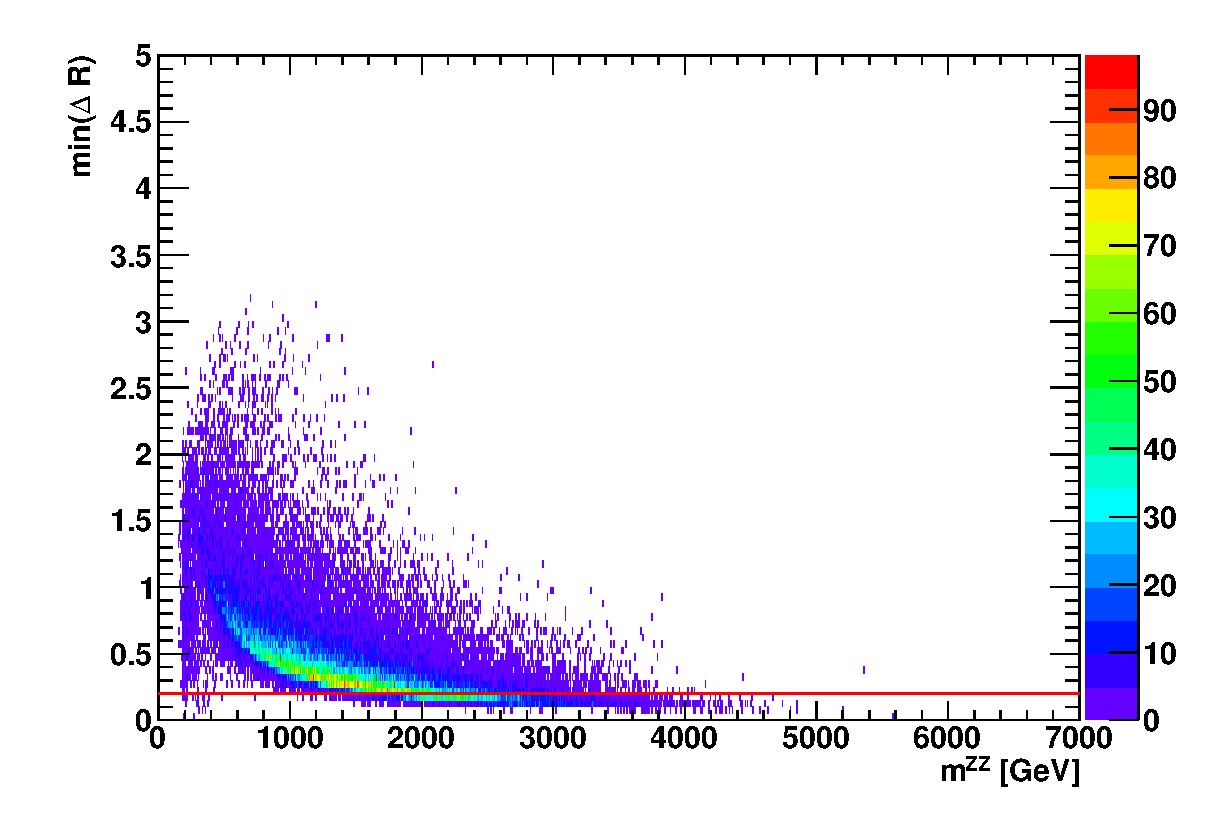
\includegraphics[width=0.7\textwidth]{deltaRcutoffs/truth_fidZZ_mzz_minDR_TGC_F4G0p4_n0}
        }
	\subfigure[]{
            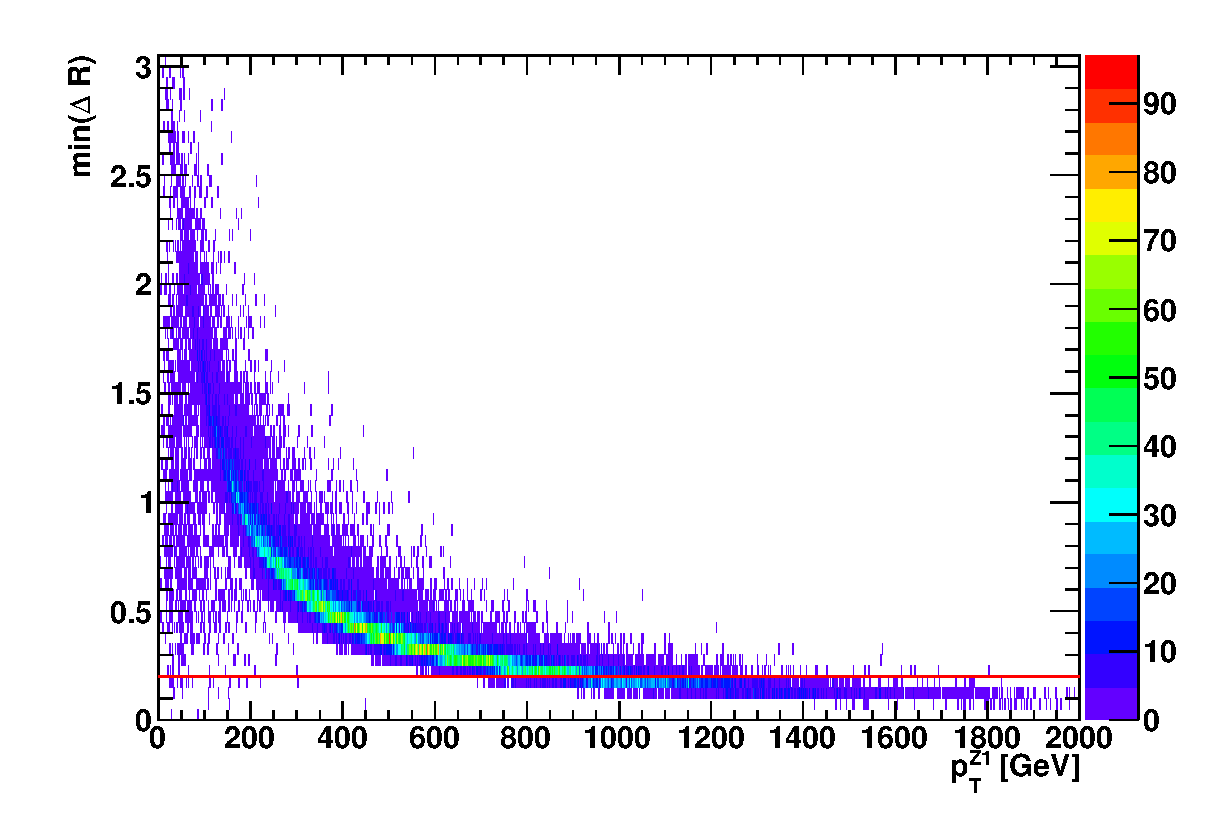
\includegraphics[width=0.7\textwidth]{deltaRcutoffs/truth_fidZZ_ptz1_minDR_TGC_F4G0p4_n0}
        }
    \caption[Effect of the \deltaRlt{0.2} requirement on sensitivity to boosted
    \fourlep\ systems.]{The minimum \deltaR\ between any two leptons, at
    generator level, in \fourlep\
    events in a \mc\ sample as a function of (a) mass of the
    \fourlep\ system and (b) transverse momentum of the leading \Z. A \ZZllll\
    sample generated with aTGCs is used, with $\ffourg=0.4$ and no form-factor
    applied, in order to give statistics at high centre
    of mass energies. The
    horizontal red line shows the \deltaRlt{0.2} cut. }
\label{fig:objSel-deltaRcutoff} 
\end{figure}

\section{Systematic Uncertainties on \CZZ}

In this section systematic uncertainties associated with the reconstruction
acceptance \CZZ\ are discussed. %The uncertainties associated with reconstruction
%and identification are discussed in Sections~\ref{sec:objSel-syst-el}
%and~\ref{sec:objSel-syst-mu}, event level

\subsection{Sources of Systematic Uncertainty}

Uncertainties arise due to the determination of
electron and muon reconstruction and identification efficiencies, the electron
and muon energy scales and resolutions, the trigger efficiency, as well as
theoretical uncertainties associated with the \mc\ simulation used to estimate
\CZZ. Each of these is discussed in more detail below.

\subsubsection{Electron Systematic Uncertainties}

\begin{itemize}
     \item {\bf Reconstruction Efficiency, Identification Efficiency:}
     Uncertainties arise from the measurement of the electron reconstruction and
     identification efficiencies. The efficiencies are measured using a `Tag and
     Probe' technique using decays of \W\, \Z\ and \JPsi. Uncertainties arise
     due to the method used to subtract the background, possible biases of the
     methodology, the definition of the
     tag electron and differences between the results from different decays, as
     well as due to the limited statistics in the data and \mc\ samples. These
     uncertainties are propagated to \CZZ\ by varying the scale-factor applied
     to the electrons up and down by its uncertainty; this is carried out
     separately for the reconstruction and identification efficiency, assuming
     the uncertainties to be uncorrelated.

    \item {\bf Energy Scale:}
    % Pre-sampler energy scale important to correct upstream energy loss. energy
    % scale calibration only gives one scale for calo measurement - the
    % presampler may have a different scale to the other layers
    Uncertainties arise on the calibration of the electron energy scale, for
    example from the different method used to measure the energy scale, the
    choice of \mc\ generator used, the uncertainty on the pre-sampler energy 
    scale, uncertainty on the amount of dead material, and differences between
    results from \Zee\ and from \JPsiee\ at low \et, as well as statistical
    uncertainties on the measurements. Whilst the energy scale calibration is
    applied to data, the systematic is estimated by varying the energy scale in
    the \mc\ up and down by the uncertainty. For the 7~\tev\ analysis, all
    uncertainties are considered at once by summing in quadrature the
    uncertainties on the scale parameter $\alpha$, whilst for 8~\tev\ each source of
    uncertainty listed above is considered separately, then the resulting
    changes in \CZZ\ are summed in quadrature.

    \item {\bf Energy Resolution:} Uncertainties arise on the measurement of the
    energy resolution in data, mainly from uncertainty on the sampling term (as the
    constant term is extracted assuming that the sampling term is correctly
    reproduced by the simulation), uncertainty on the background subtraction and
    from statistics. This is propagated to \CZZ\ by varying the width of the 
    smearing applied to the \mc\ up and down.

    \item {\bf  Isolation/\zzero/\dzero\ Efficiency:} The efficiency of the additional
    electron selection cuts (isolation, \zzero, \dzerosig) is estimated from
    data using a tag and probe technique on \Zee\ decays. The efficiency is
    consistent with that estimated by \mc\ within the uncertainties of the 
    efficiency measurement. No correction is made to the central value of the
    \mc, but the uncertainties on this efficiency, arising from uncertainties on
    the background subtraction and biases in the methodology as well as limited
    statistics, are propagated to the uncertainty on \CZZ.
     
    \item {\bf Impact Parameter Resolution:} The impact parameter
    resolution is observed to be slightly wider in data than in \mc. Whilst no
    correction is applied to the central value of the \mc, the impact of this
    effect is estimated by applying a smearing to the \mc\ to match the impact
    parameter resolution observed in data, and taking the difference in \CZZ\
    with and without the smearing as an additional systematic. This is done for
    both electrons and muons simultaneously.

\end{itemize}

\subsubsection{Muon Systematic Uncertainties}

\begin{itemize}
     \item {\bf Reconstruction Efficiency:}
     Similarly to the electrons, uncertainties arise from the measurement of the
     muon reconstruction efficiency in data.

    \item {\bf Energy Scale:} Uncertainties on the muon energy scale are
    conservatively estimated by taking the difference between the values of \CZZ\
    obtained with and without the energy scale correction applied.

    \item {\bf Energy Resolution:} The energy resolution is measured separately
    for the muon inner detector and muon spectrometer track. Uncertainties are
    estimated by varying the amount of smearing applied to the muon ID and MS
    measurements separately. 
    
    \item {\bf Isolation/\zzero/\dzero\ Efficiency:} Similarly to the electron case,
    the efficiency of the additional muon selection cuts (isolation, \zzero,
    \dzerosig) is estimated from data using a tag and probe technique on \Zmm\
    decays, and as for electrons the data and \mc\ are found to be in good
    agreement, so no correction is made to the central value of the \mc\ and
    uncertainties on the efficiency are propagated to the uncertainty on \CZZ.
\end{itemize}

\subsubsection{Trigger Systematic Uncertainty}
\subsubsection{Theoretical Systematic Uncertainty}

\subsection{Systematic Uncertainty Estimates}

\begin{table}[htbp]
   \centering
   \begin{tabular}{l|c|c|c|c}
      \hline\hline
      Source                              & \eeee           & \mmmm                  & \eemm                    & \llll                      \\
      \hline\hline
      \bf{Reconstruction Uncertainties (\%)}   & \multicolumn{4}{|c}{} \\
      \hline
      $e$ energy scale                      & \ZZSevenTeVSystematicZZEScaleEEEE           & \ZZSevenTeVSystematicZZEScaleMMMM    
                                            & \ZZSevenTeVSystematicZZEScaleEEMM           & \ZZSevenTeVSystematicZZEScaleLLLL    \\
      $e$ energy resolution                 & \ZZSevenTeVSystematicZZESmearEEEE           & \ZZSevenTeVSystematicZZESmearMMMM    
                                            & \ZZSevenTeVSystematicZZESmearEEMM           & \ZZSevenTeVSystematicZZESmearLLLL    \\
      $e$ reconstruction efficiency         & \ZZSevenTeVSystematicZZERecoEEEE            & \ZZSevenTeVSystematicZZERecoMMMM     
                                            & \ZZSevenTeVSystematicZZERecoEEMM            & \ZZSevenTeVSystematicZZERecoLLLL     \\
      $e$ identification efficiency         & \ZZSevenTeVSystematicZZEIdEEEE              & \ZZSevenTeVSystematicZZEIdMMMM       
                                            & \ZZSevenTeVSystematicZZEIdEEMM              & \ZZSevenTeVSystematicZZEIdLLLL       \\
      $e$ isolation/z0/d0Sig efficiency     & \ZZSevenTeVSystematicZZEIsoEEEE             & \ZZSevenTeVSystematicZZEIsoMMMM      
                                            & \ZZSevenTeVSystematicZZEIsoEEMM             & \ZZSevenTeVSystematicZZEIsoLLLL      \\
      $\mu$ momentum scale                  & \ZZSevenTeVSystematicZZMuScaleEEEE          & \ZZSevenTeVSystematicZZMuScaleMMMM   
                                            & \ZZSevenTeVSystematicZZMuScaleEEMM          & \ZZSevenTeVSystematicZZMuScaleLLLL   \\
      $\mu$ momentum resolution             & \ZZSevenTeVSystematicZZMuSmearEEEE          & \ZZSevenTeVSystematicZZMuSmearMMMM   
                                            & \ZZSevenTeVSystematicZZMuSmearEEMM          & \ZZSevenTeVSystematicZZMuSmearLLLL \\
      $\mu$ reconstruction efficiency       & \ZZSevenTeVSystematicZZMuRecoEEEE           & \ZZSevenTeVSystematicZZMuRecoMMMM    
                                            & \ZZSevenTeVSystematicZZMuRecoEEMM           & \ZZSevenTeVSystematicZZMuRecoLLLL    \\
      $\mu$ isolation/z0/d0Sig efficiency   & \ZZSevenTeVSystematicZZMuIsoEEEE            & \ZZSevenTeVSystematicZZMuIsoMMMM     
                                            & \ZZSevenTeVSystematicZZMuIsoEEMM            & \ZZSevenTeVSystematicZZMuIsoLLLL     \\
      Trigger                               & \ZZSevenTeVSystematicZZOverallTriggerEEEE   & \ZZSevenTeVSystematicZZOverallTriggerMMMM  
                                            & \ZZSevenTeVSystematicZZOverallTriggerEEMM   & \ZZSevenTeVSystematicZZOverallTriggerLLLL  \\
      \hline
      Total Reconstruction                  & \ZZSevenTeVSystematicZZRecoTotalEEEE        & \ZZSevenTeVSystematicZZRecoTotalMMMM 
                                            & \ZZSevenTeVSystematicZZRecoTotalEEMM        & \ZZSevenTeVSystematicZZRecoTotalLLLL \\
      \hline\hline
      \bf{Theoretical Uncertainties to \CZZ\ }      &  \multicolumn{4}{|c}{} \\
      MC Generator Difference               & \ZZSevenTeVSystematicZZGeneratorEEEE        & \ZZSevenTeVSystematicZZGeneratorMMMM 
                                            & \ZZSevenTeVSystematicZZGeneratorEEMM        & \ZZSevenTeVSystematicZZGeneratorLLLL \\
      \hline\hline
      Total \CZZ\ Uncertainty               & \ZZSevenTeVSystematicZZCzzTotalEEEE         & \ZZSevenTeVSystematicZZCzzTotalMMMM 
                                            & \ZZSevenTeVSystematicZZCzzTotalEEMM         & \ZZSevenTeVSystematicZZCzzTotalLLLL \\
      \hline\hline

   \end{tabular}
   \caption{Summary of all relative acceptance uncertainties in \% considered in the
   \zzllll\ cross-section calculation. Sums in quadrature of the weighted
   average of the three channels and a combined uncertainty are shown for the
   reconstruction uncertainties. For the PDF and scale uncertainties see
   Table~\ref{tab:MCFM} and for the uncertainty from the parton shower model see
   Section~\ref{sec:xsec}.
   %while for the differences between $gg$ and $qq$, and
   %between various generators see Table~\ref{table:CZZSherpaPythia}. 
   }
   \label{table:accSys_llll}
\end{table}
